\let\negmedspace\undefined
\let\negthickspace\undefined
\documentclass[journal]{IEEEtran}
\usepackage[a5paper, margin=10mm, onecolumn]{geometry}
%\usepackage{lmodern} % Ensure lmodern is loaded for pdflatex
\usepackage{tfrupee} % Include tfrupee package

\setlength{\headheight}{1cm} % Set the height of the header box
\setlength{\headsep}{0mm}     % Set the distance between the header box and the top of the text

\usepackage{gvv-book}
\usepackage{gvv}
\usepackage{cite}
\usepackage{amsmath,amssymb,amsfonts,amsthm}
\usepackage{algorithmic}
\usepackage{graphicx}
\usepackage{textcomp}
\usepackage{xcolor}
\usepackage{txfonts}
\usepackage{listings}
\usepackage{enumitem}
\usepackage{mathtools}
\usepackage{gensymb}
\usepackage{comment}
\usepackage[breaklinks=true]{hyperref}
\usepackage{tkz-euclide} 
\usepackage{listings}
% \usepackage{gvv}                                        
\def\inputGnumericTable{}                                 
\usepackage[latin1]{inputenc}                                
\usepackage{color}                                            
\usepackage{array}                                            
\usepackage{longtable}                                       
\usepackage{calc}                                             
\usepackage{multirow}                                         
\usepackage{hhline}                                           
\usepackage{ifthen}                                           
\usepackage{lscape}
\begin{document}

\bibliographystyle{IEEEtran}

\title{1.9.11}
\author{EE25BTECH11022 - sankeerthan}
% \maketitle
% \newpage
% \bigskip
{\let\newpage\relax\maketitle}

\renewcommand{\thefigure}{\theenumi}
\renewcommand{\thetable}{\theenumi}

\numberwithin{equation}{enumi}
\numberwithin{figure}{enumi}
\renewcommand{\thetable}{\theenumi}

\textbf{Question}: if the distance between the points $\brak{k,-2}$ and $\brak{3,-6}$ is $10$ units, find the positive value of k.

\textbf{solution}:
Let the given points be
 \begin{align}
 \vec{A} = \myvec{k \\ -2}, \vec{B} = \myvec{3 \\ -6} 
 \end{align}
The direction vector of the segment joining A and B is given by:
\begin{align}
\vec{B} - \vec{A} = \myvec{3 - k \\ -6 -(-2)} = \myvec{3-k \\ -4} 
\end{align}
The length of the segment is the magnitude of the direction vector:
 \begin{align}
\vec{B} - \vec{A} = \myvec{3 - k \\ -6 -(-2)} = \myvec{3-k \\ -4} 
\end{align}
The distance between points $\vec{A}$ and $\vec{B}$ is given as,
d = $\|\vec{B-A}\|$ = 10
\begin{align}
\|\vec{B-A}\| = \sqrt{\brak{\vec{B}-\vec{A}}^\top \brak{\vec{B}-\vec{A}}}  \\
\brak{\vec{B}-\vec{A}}^\top \brak{\vec{B}-\vec{A}} = \|\vec{B-A}\|^2
\brak{\vec{B}-\vec{A}}^\top \brak{\vec{B}-\vec{A}} = (10)^2
\end{align}
\begin{align}
100 &=\myvec{3-k  \ -4}\myvec{3-k \\ -4}\\
100 &=(3-k)\times(3-k)+(-4)\times(-4) \\
100 &=(3-k)^2 + 16 \\
(3-k)^2 &= 84 \\
3-k &=\pm \sqrt{84} \\
k &= 3+\sqrt{84} ,3-\sqrt{84}
\end{align}

Therefore, the positive value of k is $3+\sqrt{84} \approx 12.17$

\begin{figure}
   \centering
   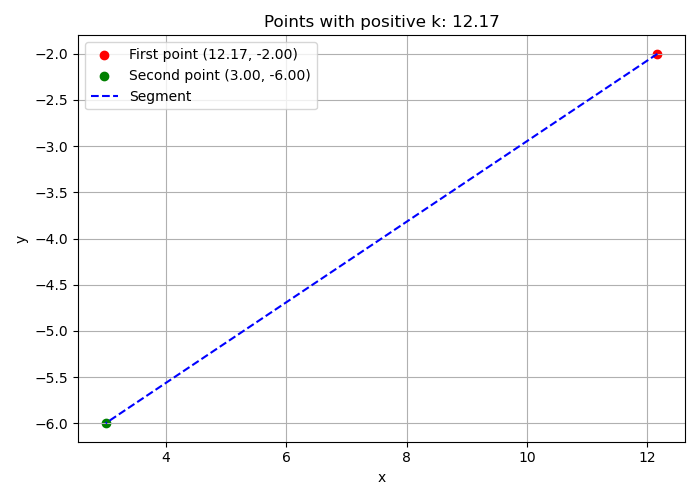
\includegraphics[width=1\columnwidth]{figs/points.png}
   \caption{Plot of line segment \textbf{AB}}
   \label{}
\end{figure}
\end{document}